
\begin{figure}
    \centering
    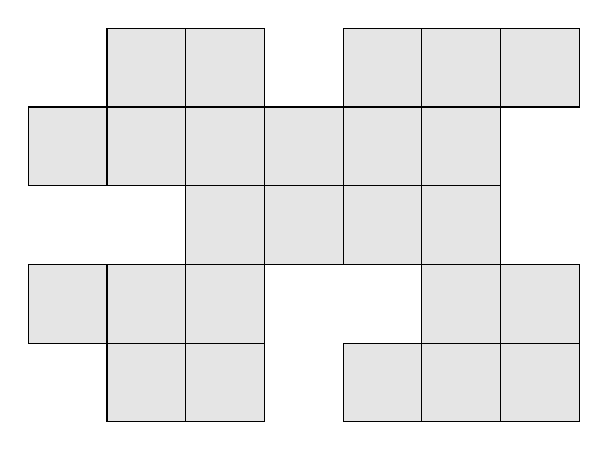
\begin{tikzpicture}
        \tikzstyle{cell} = [draw, thick, minimum size=1cm]

		\draw[fill=gray!20, draw=black] (1,0) rectangle (2,-1);
		\draw[fill=gray!20, draw=black] (2,0) rectangle (3,-1);
		\draw[fill=gray!20, draw=black] (4,0) rectangle (5,-1);
		\draw[fill=gray!20, draw=black] (5,0) rectangle (6,-1);
		\draw[fill=gray!20, draw=black] (6,0) rectangle (7,-1);
		\draw[fill=gray!20, draw=black] (0,-1) rectangle (1,-2);
		\draw[fill=gray!20, draw=black] (1,-1) rectangle (2,-2);
		\draw[fill=gray!20, draw=black] (2,-1) rectangle (3,-2);
		\draw[fill=gray!20, draw=black] (3,-1) rectangle (4,-2);
		\draw[fill=gray!20, draw=black] (4,-1) rectangle (5,-2);
		\draw[fill=gray!20, draw=black] (5,-1) rectangle (6,-2);
		\draw[fill=gray!20, draw=black] (2,-2) rectangle (3,-3);
		\draw[fill=gray!20, draw=black] (3,-2) rectangle (4,-3);
		\draw[fill=gray!20, draw=black] (4,-2) rectangle (5,-3);
		\draw[fill=gray!20, draw=black] (5,-2) rectangle (6,-3);
		\draw[fill=gray!20, draw=black] (0,-3) rectangle (1,-4);
		\draw[fill=gray!20, draw=black] (1,-3) rectangle (2,-4);
		\draw[fill=gray!20, draw=black] (2,-3) rectangle (3,-4);
		\draw[fill=gray!20, draw=black] (5,-3) rectangle (6,-4);
		\draw[fill=gray!20, draw=black] (6,-3) rectangle (7,-4);
		\draw[fill=gray!20, draw=black] (1,-4) rectangle (2,-5);
		\draw[fill=gray!20, draw=black] (2,-4) rectangle (3,-5);
		\draw[fill=gray!20, draw=black] (4,-4) rectangle (5,-5);
		\draw[fill=gray!20, draw=black] (5,-4) rectangle (6,-5);
		\draw[fill=gray!20, draw=black] (6,-4) rectangle (7,-5);

    \end{tikzpicture}
    \caption{xxx}
    \label{fig:xxx}
\end{figure}
